\documentclass[aspectratio=169, 13pt]{beamer}
\usepackage[utf8]{inputenc}
\usepackage[english,russian]{babel}
\usepackage{graphicx}
\usepackage{sidecap}
\usepackage{mathtools}
\usepackage{appendixnumberbeamer}
\usepackage{bbm}

\newcommand{\sbrkt}[1]{\left[ #1 \right]}
\DeclarePairedDelimiter\bra{\langle}{\rvert}
\DeclarePairedDelimiter\ket{\lvert}{\rangle}
\DeclarePairedDelimiterX\braket[2]{\langle}{\rangle}{#1 \delimsize\vert #2}
\newcommand{\rbrkt}[1]{\left( #1 \right)}
\newcommand{\lbrkt}[1]{\left< #1 \right>}


\graphicspath{{../Pictures/}}
\graphicspath{{../Pictures2/}}

%beamer  theme's used to be here :)
\usetheme{mipt_beamer}
\usefonttheme[onlymath]{serif}

\title{Исследование сверхпроводящих потоковых кубитов}
\author{Сафронов~Е.~С. Группа 325. \quad Научный руководитель: Шульга~К.В.}
\date{\today}

\setlength{\jot}{15pt}
\setbeamertemplate{footline}[page number]
\renewcommand*{\inserttotalframenumber}{\insertpresentationendpage}
\newcommand{\Tr}[1]{\text{Tr}\left[#1\right]}

\AtBeginSection[]
{
  \begin{frame}[plain]
    \tableofcontents[currentsection]
    \addtocounter{page}{-1}
  \end{frame}
}



\begin{document}

{
\begin{frame}[plain]
  \titlepage
\end{frame}
}

\frame[plain]{\tableofcontents}

\section{Основы}
\subsection{Кубит и его представления}
\begin{frame}[c]\frametitle{\secname}\framesubtitle{\subsecname}

\begin{columns}[c]
\column{0.35\textwidth}
\centering
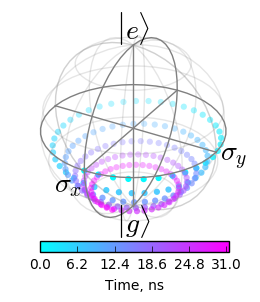
\includegraphics[width=0.95\textwidth]{bloch_sphere_dissipative}

Диссипативная траектория на сфере Блоха

\column{0.05\textwidth}
\vspace{5cm}
$\leftarrow$
\column{0.23 \textwidth}
\centering
\begin{gather*}
\hat \rho = \frac{1}{2}(\mathbbm{\hat 1} + a\hat \sigma_x+b\hat \sigma_y + c\hat \sigma_z)
\end{gather*}
\begin{gather*}
\ket{\psi} = \alpha \ket{e} + \beta \ket{g}
\end{gather*}

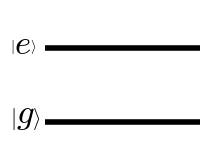
\includegraphics[width=0.8\textwidth]{two_level_transmon}
\vspace{2cm}
\column{0.05 \textwidth}
\vspace{-0.8cm}
$\in$


\column{0.27\textwidth}
\centering
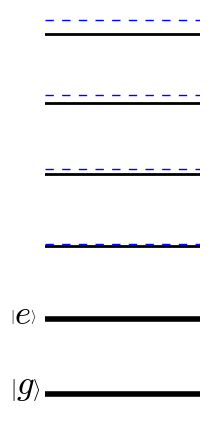
\includegraphics[width=0.8\textwidth]{many_level_transmon}

\vspace{0.1cm}
``Искусственный атом''

\end{columns}
\end{frame}

\subsection{Операции над кубитами}
\begin{frame}[c]\frametitle{\secname}\framesubtitle{\subsecname}


\end{frame}


\subsection{Источники ошибок}
\begin{frame}[c]\frametitle{\secname}\framesubtitle{\subsecname}


\end{frame}


\subsection{Система из двух кубитов}
\begin{frame}[c]\frametitle{\secname}\framesubtitle{\subsecname}


\end{frame}


\section{Методы}

\subsection{N-уровневая модель трансмона}
\begin{frame}[c]\frametitle{\secname}\framesubtitle{\subsecname}


\end{frame}

\subsection{DRAG, Half-Derivative}
\begin{frame}[c]\frametitle{\secname}\framesubtitle{\subsecname}


\end{frame}

\subsection{GRAPE}
\begin{frame}[c]\frametitle{\secname}\framesubtitle{\subsecname}


\end{frame}

\section{Результаты}
\subsection{Оптимизация однокубитных импульсов}
\begin{frame}[c]\frametitle{\secname}\framesubtitle{\subsecname}


\end{frame}

\subsection{Оптимизация однокубитных импульсов}
\begin{frame}[c]\frametitle{\secname}\framesubtitle{\subsecname}


\end{frame}

\subsection{Controlled Phase gate}
\begin{frame}[c]\frametitle{\secname}\framesubtitle{\subsecname}


\end{frame}

\subsection{Controlled NOT gate}
\begin{frame}[c]\frametitle{\secname}\framesubtitle{\subsecname}


\end{frame}

\section{Заключение}
\begin{frame}[c]\frametitle{\secname}\framesubtitle{\subsecname}


\end{frame}

\iffalse


Состояние классического бита:
\begin{equation*}
0\ \text{или}\ 1
\end{equation*}
Состояние квантового бита:
\hspace{-2cm}
\begin{gather*}
\hat \rho = \frac{1}{2}(\mathbbm{\hat 1} + a\hat \sigma_x+b\hat \sigma_y + c\hat \sigma_z),\ a,b,c \in \mathbb{R},\\
a^2 + b^2 + c^2 \in [0, 1]\\
\mathbf{r} = \rbrkt{\begin{matrix}a\\ b\\ c \end{matrix}} -\text{вектор внутри единичного шара}
\end{gather*}




\subsection{Теория изолированного Flux-кубита}
\begin{frame}[c]\frametitle{\secname}\framesubtitle{\subsecname}

\vspace{-1cm}
\only<1>{

\vspace{0.5cm}
Степени свободы: 
\begin{equation*}
\varphi_1,\ \varphi_2,\ \varphi_3 = 2\pi\frac{\Phi}{\Phi_0} - \varphi_1 - \varphi_2 \ (\text{квантование }\Phi,\ \varphi_3\ \text{зависима от первых двух})
\end{equation*}
}

\only<1>{
\begin{columns}[c]
\column{0.5\textwidth}
Энергия одного перехода:
\hspace{-1cm}
\begin{align*}
E_i = E_J(1-\cos\varphi_i) + \frac{\hbar^2}{4E_C} \dot \varphi_i^2, \\ 
E_J = \frac{\hbar}{2e}I_c,\ E_C = \frac{(2e)^2}{2C}
\end{align*}

\column{0.5\textwidth}
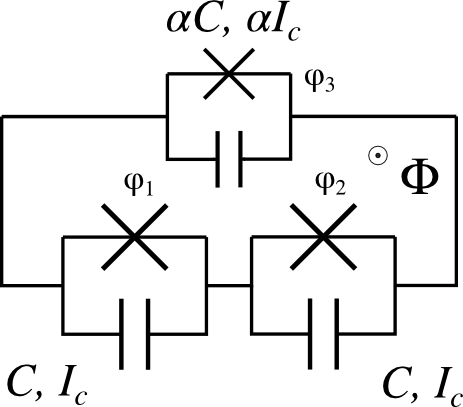
\includegraphics[width = 0.75\textwidth]{qubit}

\end{columns}
}
\only<2>{

\begin{columns}[t]
\column{0.5\textwidth}

\vspace{1cm}
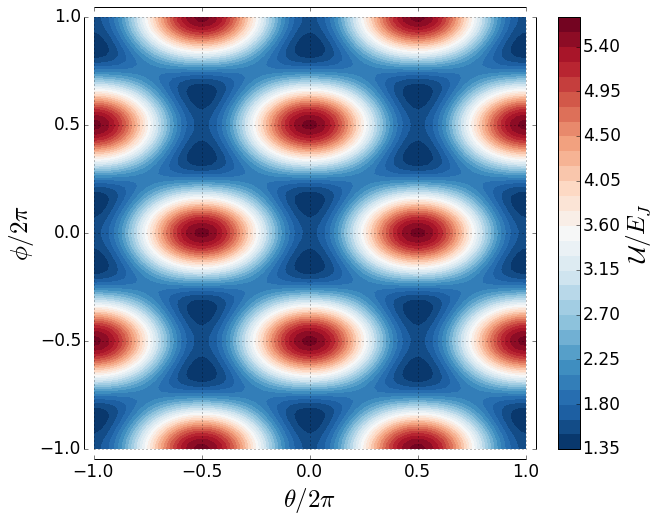
\includegraphics[width=\textwidth]{qubit_potential}

\column{0.5\textwidth}

\vspace{1cm}
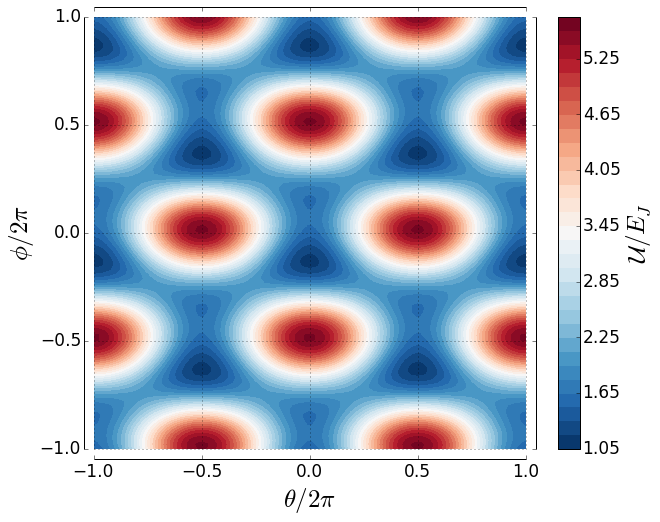
\includegraphics[width=\textwidth]{qubit_potential2}

\end{columns}

\begin{gather*}
 U = E_J\bigg[2+\alpha - 2\cos(\phi)\cos(\theta) 
-\left. \alpha\cos\left(2\pi\frac{\Phi}{\Phi_0} -2\phi \right)\right], \phi = \frac{\varphi_1+\varphi_2}{2}, \theta=\frac{\varphi_1 - \varphi_2}{2}
\end{gather*}
}

\end{frame}

\begin{frame}[c]\frametitle{\secname}\framesubtitle{\subsecname}
\only<1>{
\begin{columns}[c]

\column{\textwidth}

\vspace{0cm}
\centering
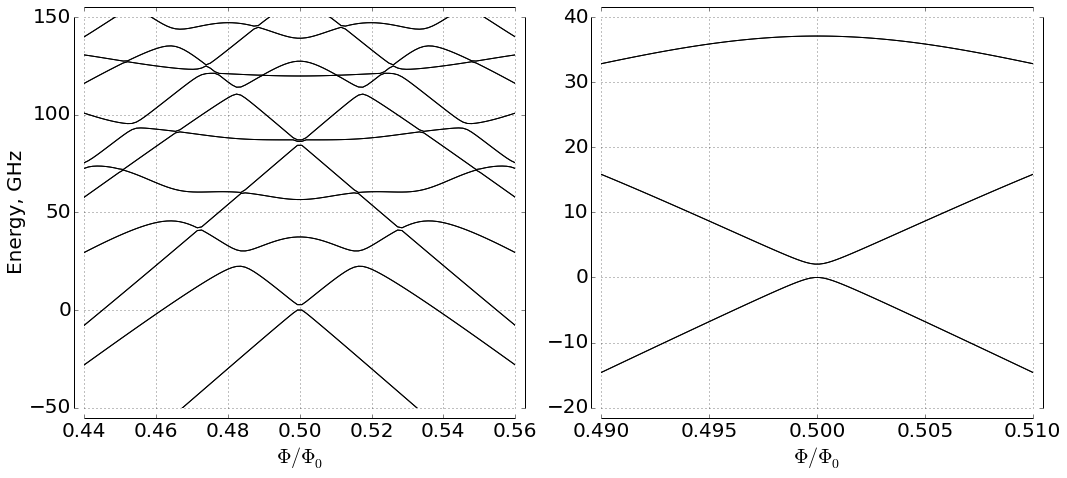
\includegraphics[width=0.7\textwidth]{qubit_levels}
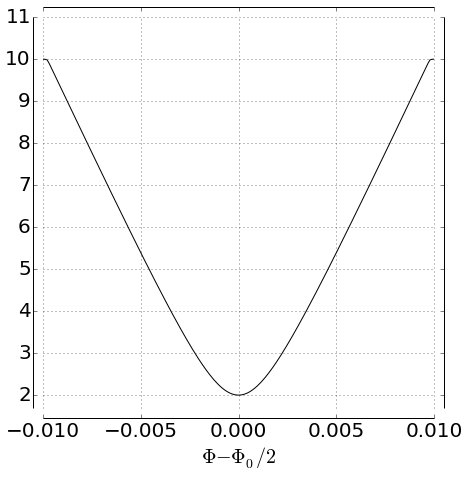
\includegraphics[width=0.307\textwidth]{spectrum_hyp}
\begin{gather*}
\hat{\mathcal{H}} = \frac{\hbar\Delta}{2}\,\hat\sigma_z + \frac{\hbar\varepsilon}{2}\,\hat\sigma_x,\ 
E_1 - E_0 = \hbar\sqrt{\Delta^2+\varepsilon^2} \text{ -- гипербола по }\delta
 \\ \small{ \ket{0}_{\Phi_0/2}=\rbrkt{\begin{matrix}
1 & 0\end{matrix}}^T,\ \ket{1}_{\Phi_0/2}=\rbrkt{\begin{matrix}
0 & 1\end{matrix}}^T,\ \delta \propto \Phi-\Phi_0/2}
\end{gather*}
\end{columns}
}
\end{frame}


\subsection{Кубит, связанный с резонатором}
\begin{frame}[c]\frametitle{\secname}\framesubtitle{\subsecname}
\begin{columns}[c]

\column{0.5\textwidth}
\centering
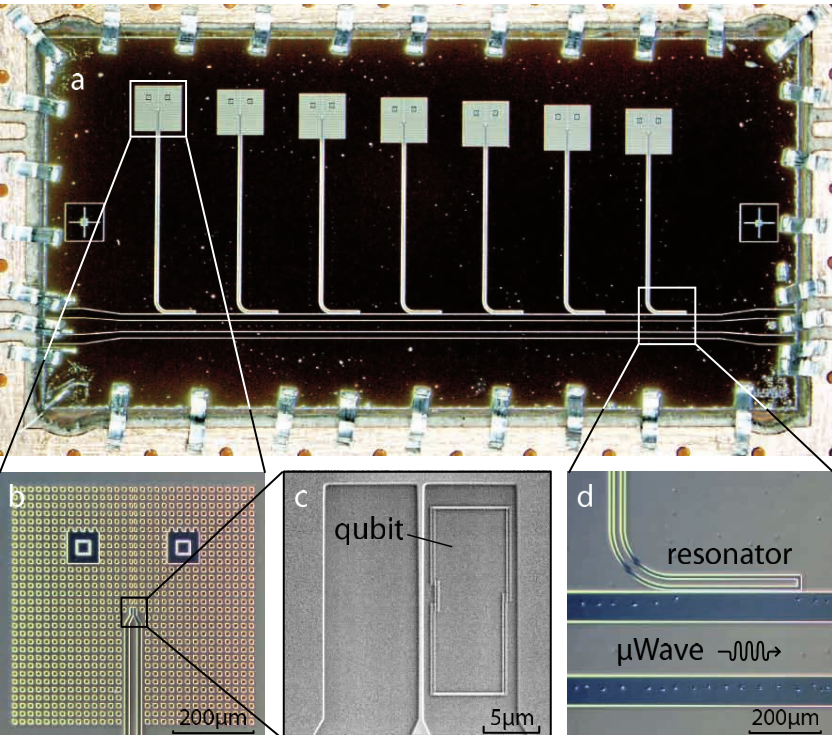
\includegraphics[width=\textwidth]{marcus_chip}
\column{0.5\textwidth}
Ситуация при $\Phi = \Phi_0/2$:
\begin{gather*}
\hat{\mathcal{H}} = \hat{\mathcal{H}}_{q}+\hat{\mathcal{H}}_{r}+\hat{\mathcal{H}}_{i},\\
\hat{\mathcal{H}}_{q} = \frac{\varepsilon}{2} \hat{\sigma_z} = \frac{\hbar\omega_q}{2}\hat{\sigma_z},\\
\hat{\mathcal{H}}_{r} = \hbar\omega_r \hat a^+ \hat{a}, \\
\hat{\mathcal{H}}_{i} = 
\begin{cases} 
\hbar g(\hat a^\dag + \hat{a})\hat{\sigma}_x = \hbar g(\hat a^\dag + \hat{a})(\hat\sigma^++\hat\sigma^-) \\ 
\hbar g(\hat a^\dag \hat\sigma^- + \hat{a}\hat\sigma^+)\ \text{-- первый порядок}
\end{cases}
\end{gather*}
Две модели: Раби (без приближений) и Джейнса-Каммингса (приближенная)

\end{columns}
\end{frame}

\subsection{Уровни энергии и спектр}

\begin{frame}[c]\frametitle{\secname}\framesubtitle{\subsecname}
\begin{columns}[c]
\column{0.5\textwidth}
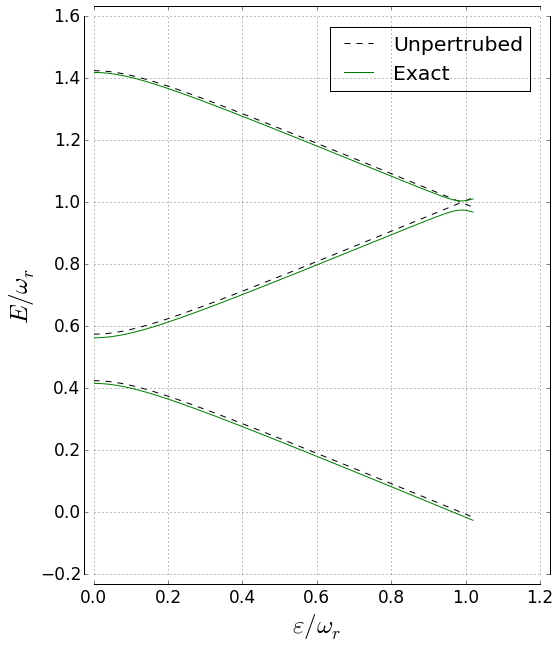
\includegraphics[height=0.85\textheight]{Rabi_levels}
\column{0.5\textwidth}
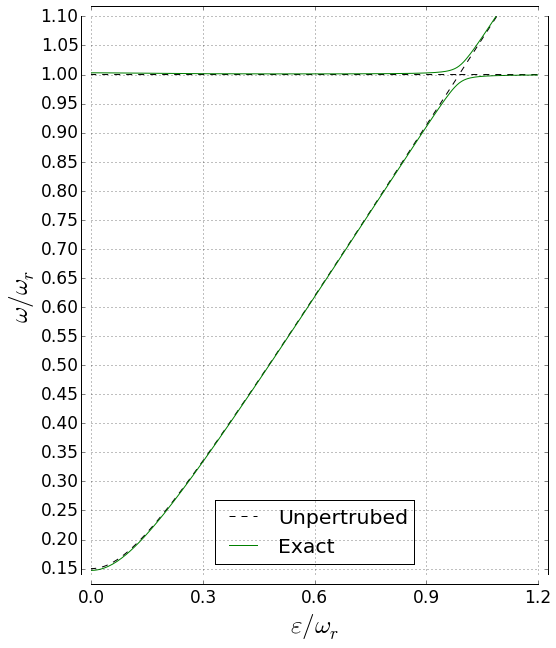
\includegraphics[height=0.85\textheight]{Rabi_spectrum}
\end{columns}
\end{frame}

\begin{frame}[c]\frametitle{\secname}\framesubtitle{\subsecname}
\centering
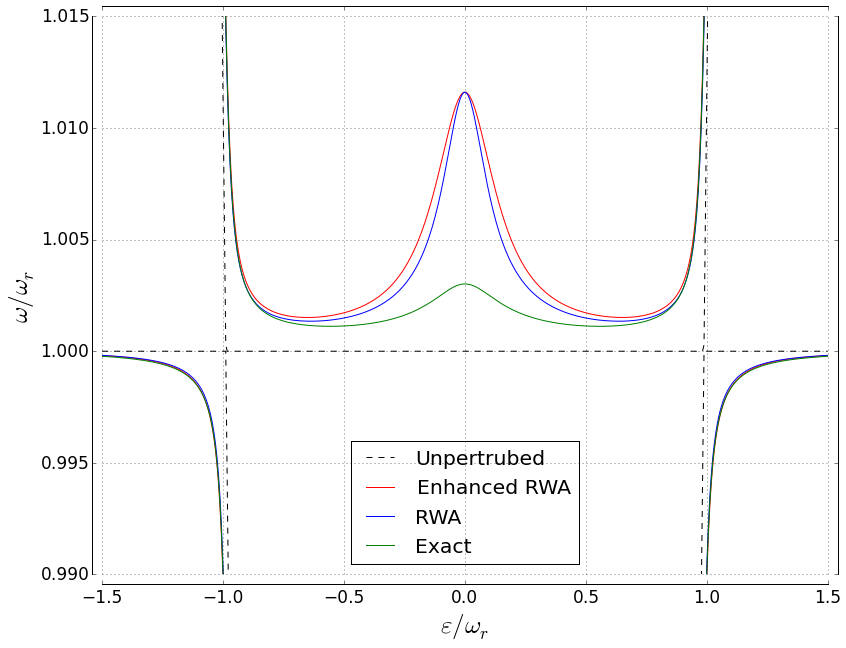
\includegraphics[width=0.7\textwidth]{Rabi_anticrossing}
\end{frame}

\section{Экспериментальные методы}
\subsection{Установка}
\frame{\frametitle{\secname}\framesubtitle{\subsecname}
\begin{columns}[c]
\column{\textwidth}
Взаимодействие с образцом внутри криостата:
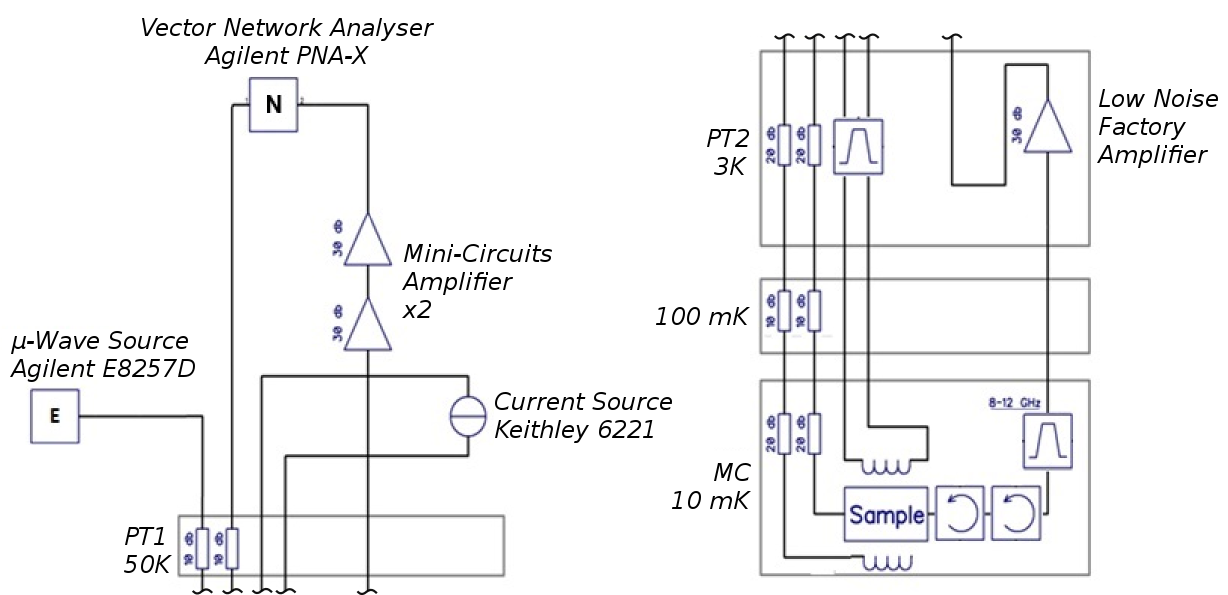
\includegraphics[width=\textwidth]{crio_scheme}
\end{columns}
}
\subsection{Техника измерений}
\frame{\frametitle{\secname}\framesubtitle{\subsecname}
\begin{columns}[c]
\column{0.5\textwidth}

В эксперименте наблюдаются сдвиги или расщепления частот поглощения:

\vspace{0.2cm}
\begin{center}
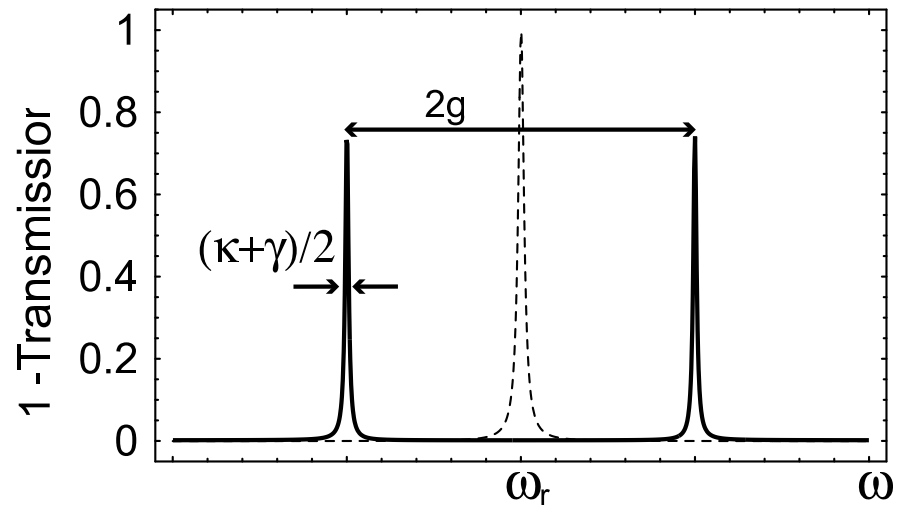
\includegraphics[width=\textwidth]{frequency_shift}
\end{center}

Черные стрелки соответствуют линиям на графике пропускания
\column{0.5\textwidth}
\centering

Иллюстрация однотоновой и двухтоновой спектроскопий:

\vspace{0.2cm}
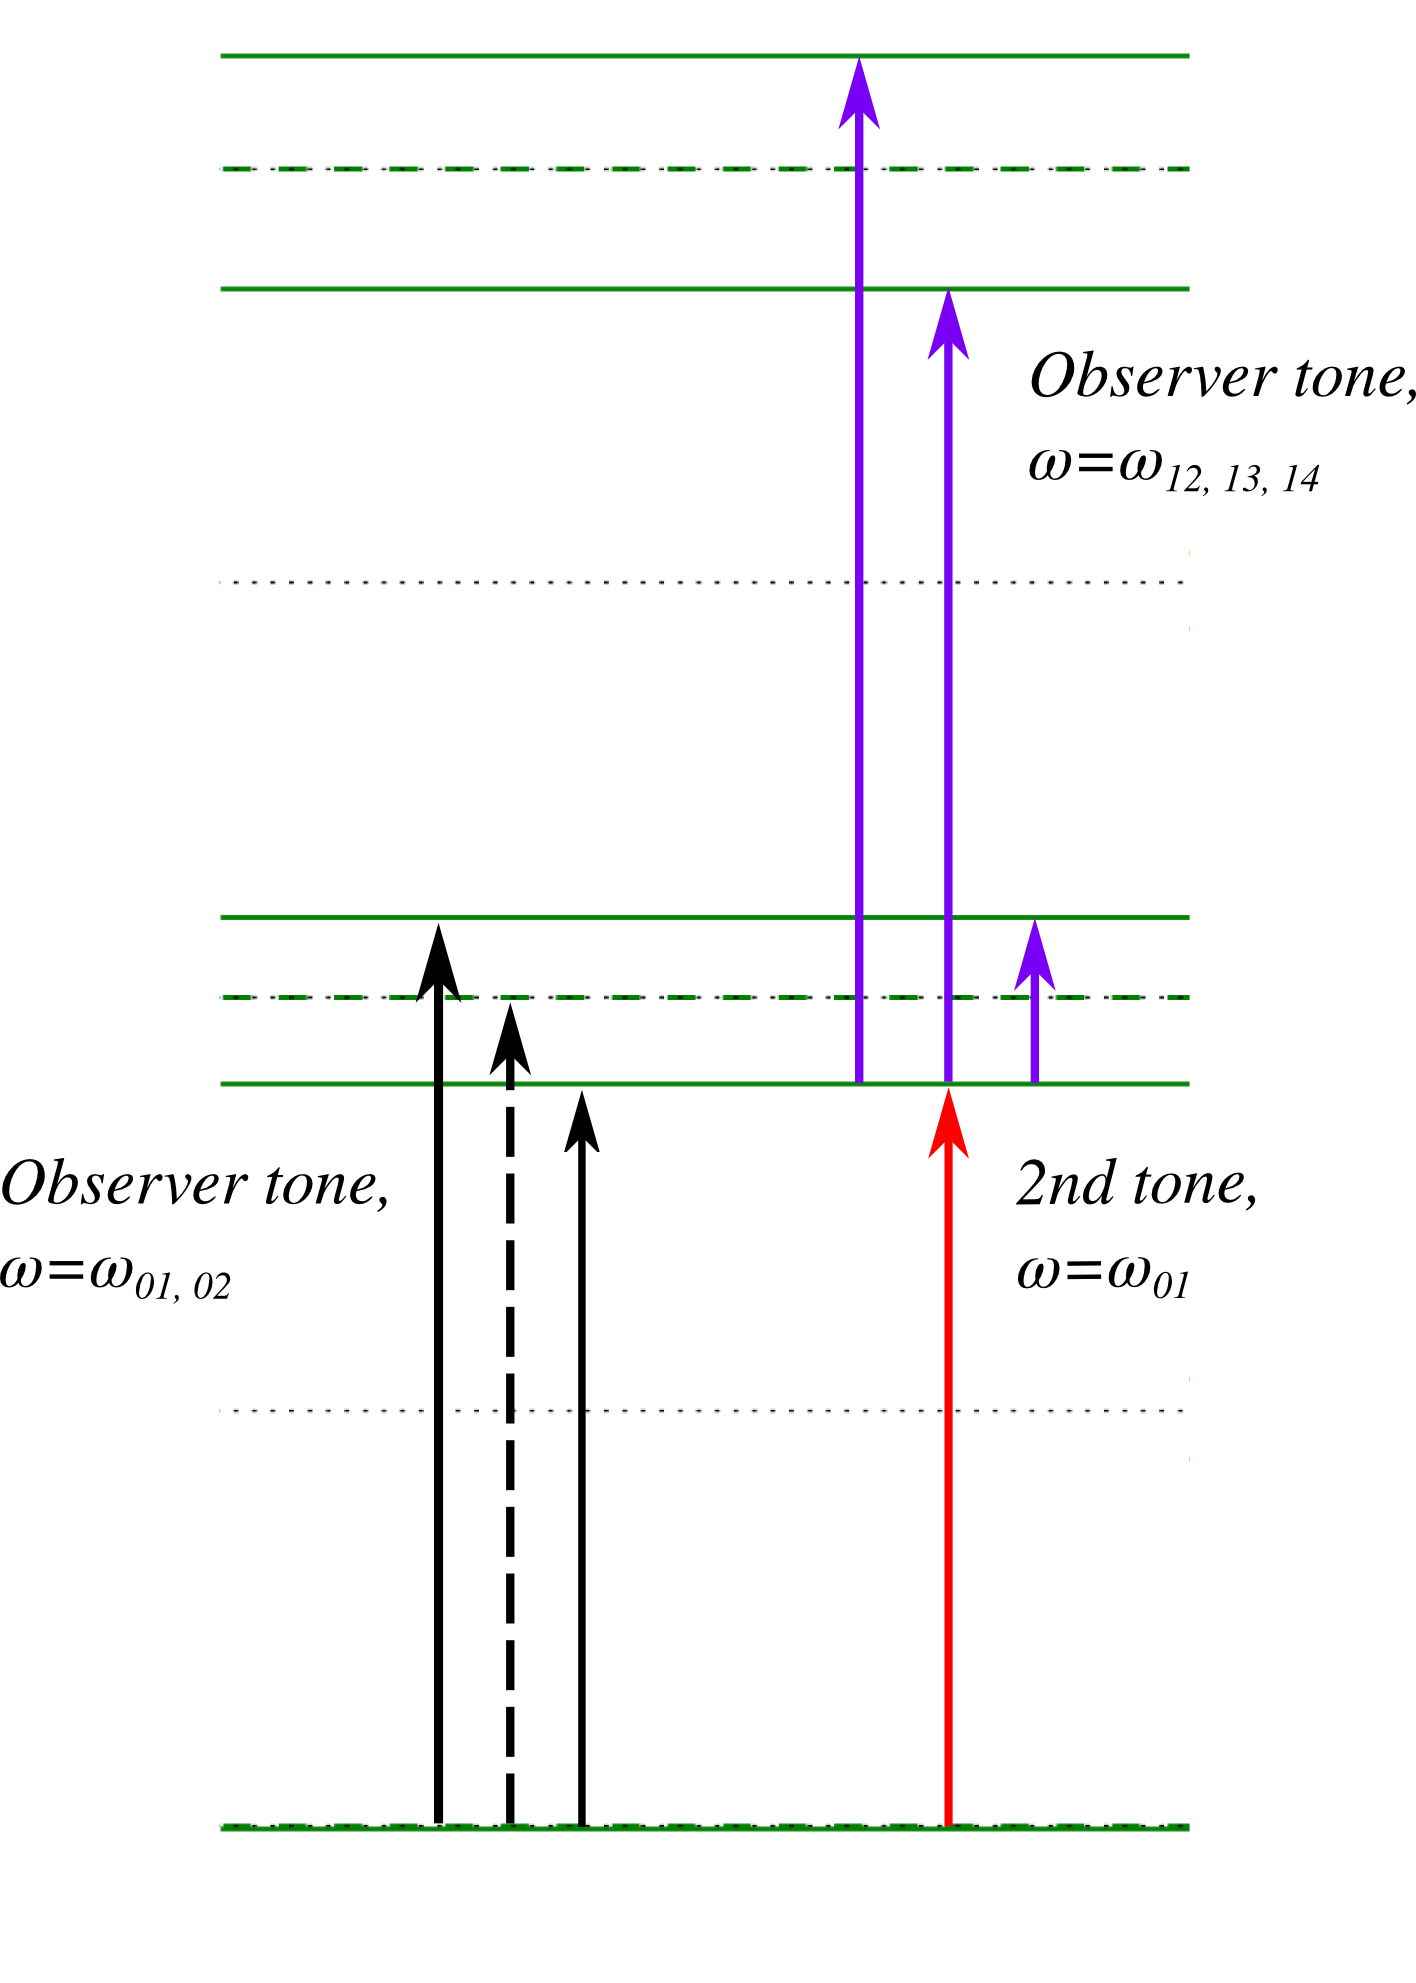
\includegraphics[height=0.75\textheight]{2tone}

\end{columns}
}

\subsection{Двухтоновая спектроскопия}
\begin{frame}[c]\frametitle{\secname}\framesubtitle{\subsecname}
\begin{columns}[c]
\column{0.5\textwidth}
\centering
Теория:

\vspace{1cm}
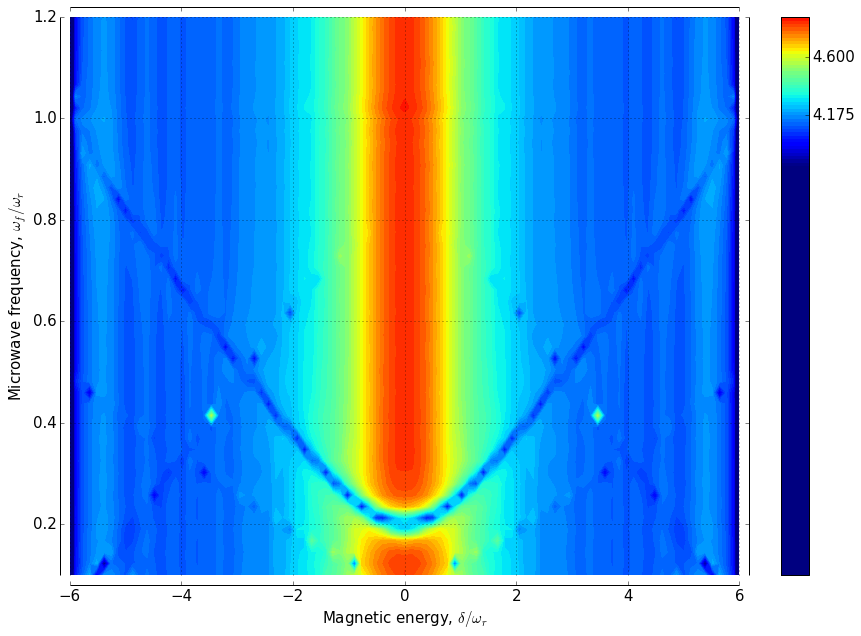
\includegraphics[width=0.9\textwidth]{two_tone}

\column{0.5\textwidth}
\centering
Эксперимент:

\vspace{1cm}
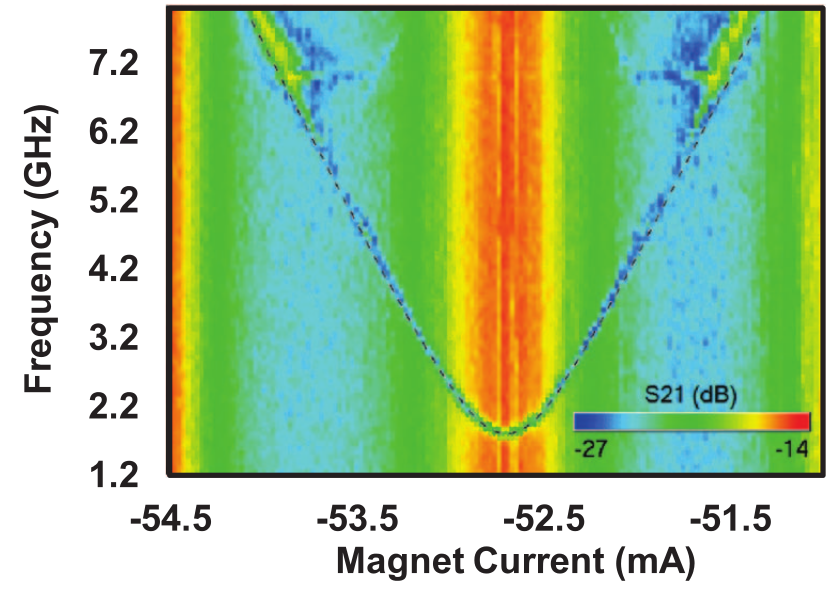
\includegraphics[width=0.9\textwidth]{sin}

\end{columns}
\end{frame}

\section{Результаты}
\subsection{Двухтоновые спектры малой мощности}
\frame{\frametitle{\secname}\framesubtitle{\subsecname}

\vspace{0.5cm}
\begin{columns}[t]

\column{0.3\textwidth}
\centering
Второй резонатор/кубит

\vspace{0.2cm}
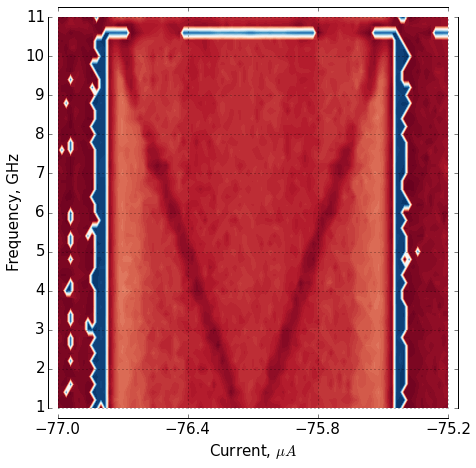
\includegraphics[width=\textwidth]{two-tone_spectrum1}

\column{0.3\textwidth}
\centering
Пятый резонатор/кубит

\vspace{0.2cm}
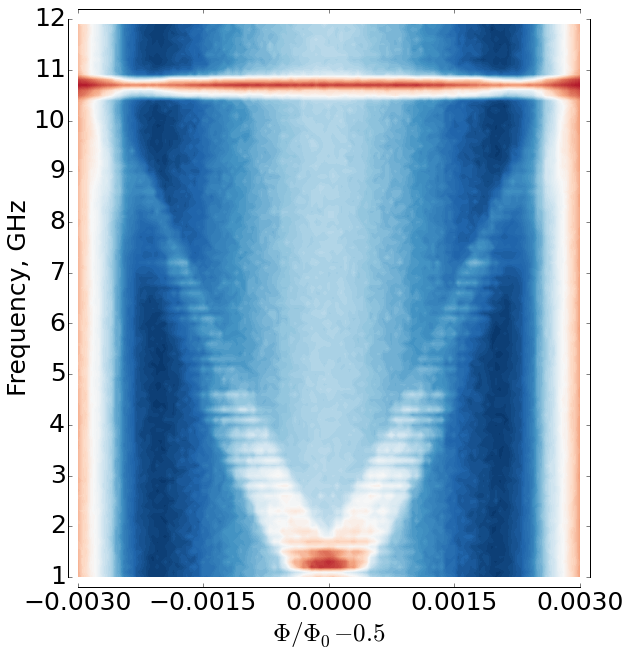
\includegraphics[width=\textwidth]{two-tone_spectrum3}

\column{0.3\textwidth}
\centering
Пятый резонатор/кубит

\vspace{0.2cm}
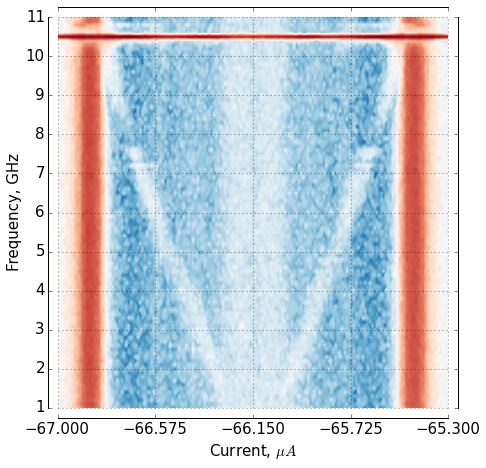
\includegraphics[width=\textwidth]{two-tone_spectrum2}

\end{columns}

\vspace{0.5cm}
Гиперболическая зависимость от $\varepsilon\propto \Phi - \Phi_0/2$:
\centering
\begin{equation*}
\hbar \omega_q = \hbar\sqrt{\varepsilon^2+\Delta^2}
\end{equation*}
}


\subsection{Двухтоновая спектроскопия большой мощности}
\frame{\frametitle{\secname}\framesubtitle{\subsecname}
\begin{columns}[c]
\column{0.5\textwidth}
\centering
Без вычитания фона:

\vspace{0.2cm}
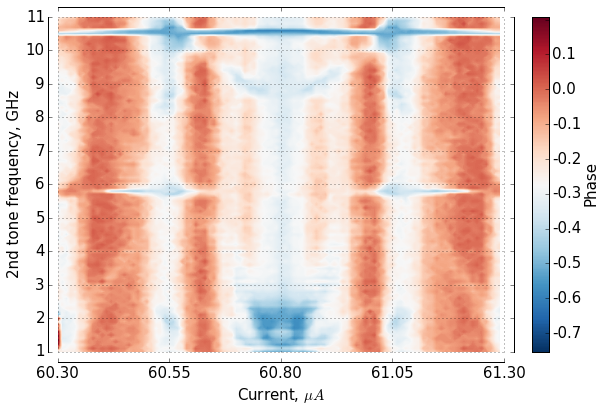
\includegraphics[width=0.9\textwidth]{two-tone_spectrum_highpower}
\column{0.5\textwidth}
\centering
Без фона:

\vspace{0.2cm}
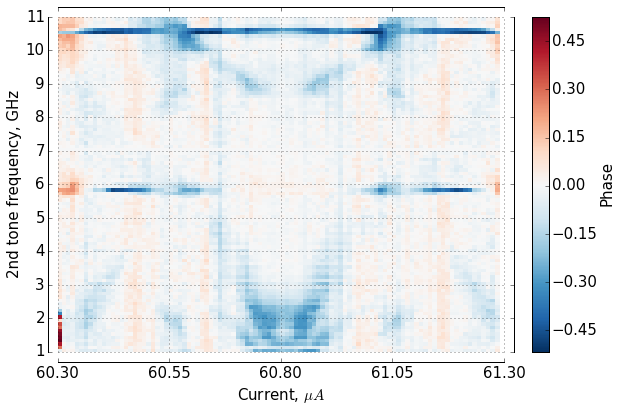
\includegraphics[width=0.9\textwidth]{two-tone_spectrum_highpower_nb}
\end{columns}

\vspace{0.5cm}
\begin{columns}[c]
\column{0.4\textwidth}
Обнаруживаются переходы:
\column{0.6\textwidth}
$\ket{0,0,g}\rightarrow\ket{0,0,e}$ -- одно- и двухфотонный

$\ket{0, 0, e}\rightarrow\ket{1, 0, g}$ -- однофотонный

$\ket{0, 0, g}\rightarrow\ket{1,1,e}$ -- двухфотонный
\end{columns}
}
\subsection{Квазипересечения спектров (пятый кубит)}
\frame{\frametitle{\secname}\framesubtitle{\subsecname}

Спектры переходов $\ket{0}\rightarrow\ket{1}$ и $\ket{0}\rightarrow\ket{2}$:

\vspace{0.5cm}
\begin{columns}[c]
\column{0.5\textwidth}
\centering
Теория:

\vspace{0.2cm}
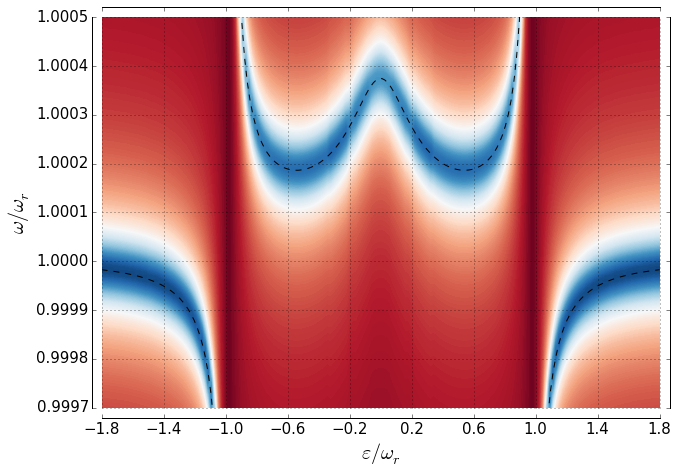
\includegraphics[width=0.9\textwidth]{anticrossing_double1}
\column{0.5\textwidth}
\centering
Эксперимент:

\vspace{0.2cm}
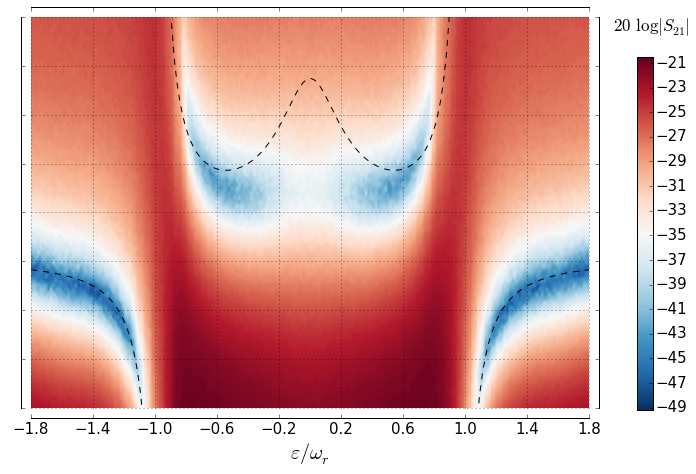
\includegraphics[width=0.9\textwidth]{anticrossing_double2}
\end{columns}

\begin{center}
\vspace{0.2cm}
Поведение исследовавшегося образца отклоняется от смоделированного поведения модели Раби в верхней ветви ($\ket{0}\rightarrow\ket{2}$).
\end{center}
}
\frame{\frametitle{\secname}\framesubtitle{\subsecname}
Увеличенный снимок левого квазипересечения:

\vspace{0.5cm}
\begin{columns}[c]
\column{0.5\textwidth}
\centering
Теория:

\vspace{0.2cm}
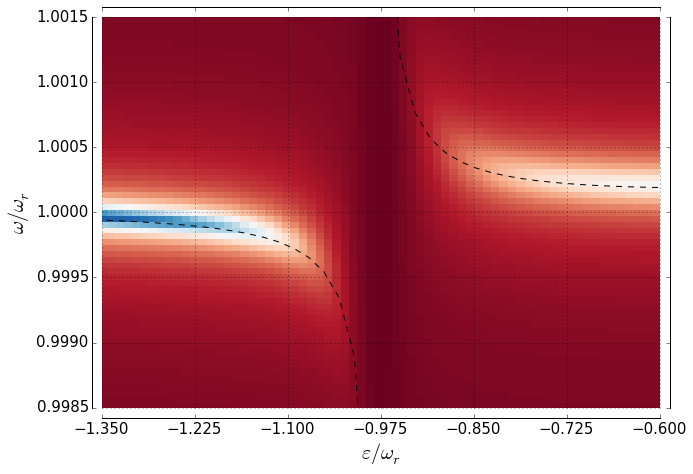
\includegraphics[width=0.95\textwidth]{anticrossing_vanishing} 
\column{0.5\textwidth}
\centering
Эксперимент:

\vspace{0.2cm}
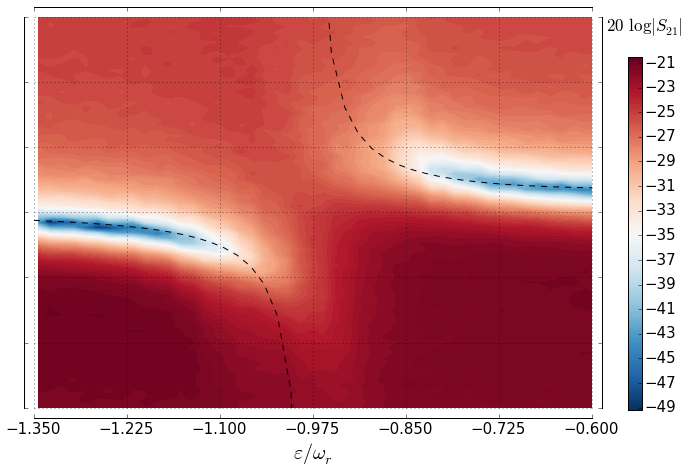
\includegraphics[width=0.95\textwidth]{anticrossing_vanishing_exp}
\end{columns}

\vspace{0.2cm}
\begin{center}
Моделирование показывает, что ненаблюдаемость квазипересечения связана с малым времени жизни кубита
\end{center}
}
\subsection{Нелинейные эффекты}
\frame{\frametitle{\secname}\framesubtitle{\subsecname} 
\begin{columns}[c]
\column{0.65\textwidth}
\centering
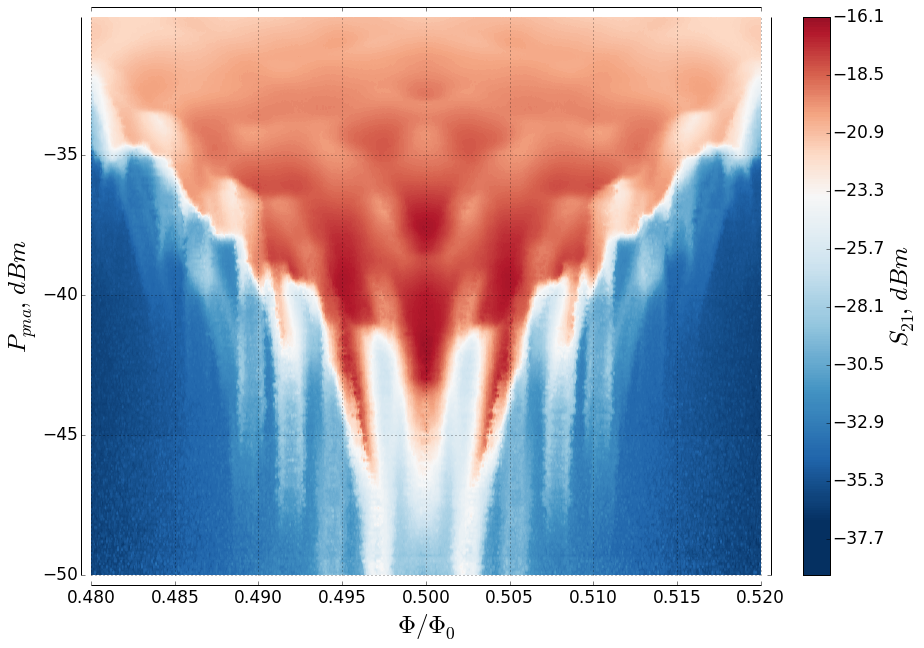
\includegraphics[width=\textwidth]{LZI}
\column{0.35\textwidth}
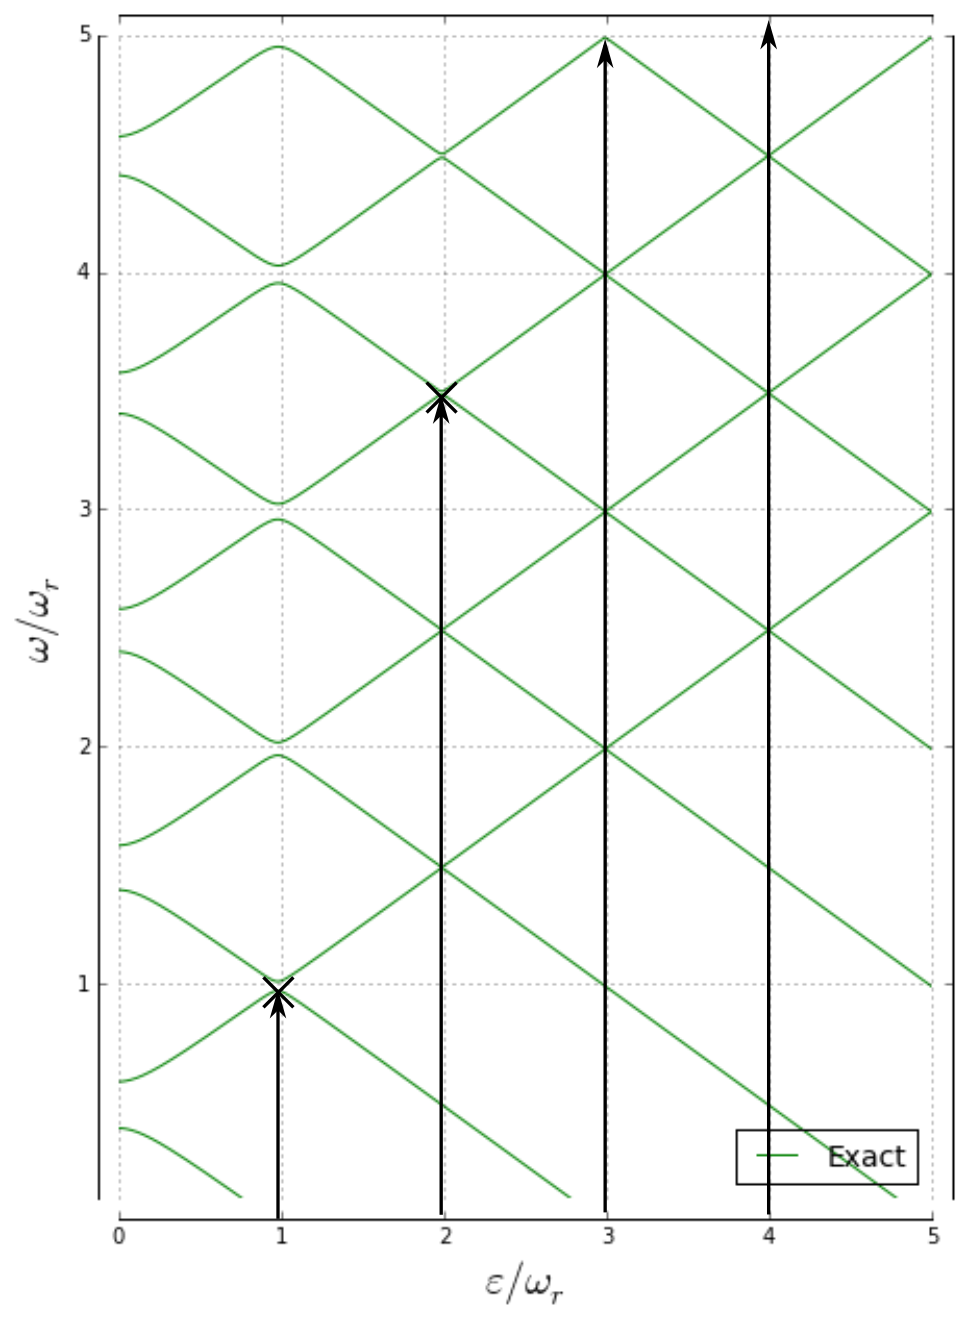
\includegraphics[width=\textwidth]{JCM_MF}

\end{columns}
}

\section{Заключение}

\frame{\frametitle{\secname}\framesubtitle{Главные результаты} 

\begin{enumerate}
\item Численное моделирование широкого класса эффектов, связанных со стационарным и динамическим поведением исследуемой системы. 

\item По ширине линий спектров оценены времена жизни кубитов. Изучена структура уровней исследуемой системы кубит-резонатор при проведении двухтоновой спектроскопии высокой мощности.

\item Исследованы квазипересечения спектров кубита и резонатора, результаты сравнены с результатами выполненного численного моделирования.

\item Проведены наблюдения нелинейных по мощности эффектов в поведении зависимости пропускания на частоте резонатора  от тока, эффекты объяснены.

\end{enumerate}
}

\appendix

\section*{Вспомогательные материалы}
\subsection*{Сверхпроводимость и эффект Джозефсона}
\begin{frame}[noframenumbering, c, label=1st]\frametitle{\secname}\framesubtitle{\subsecname}
\addvspace{-2cm}

\begin{columns}[c]
\column{0.5\textwidth}

\vspace{1.2cm}
\only<1>{Теория Г.-Л. и уравнения Джозефсона:}
\only<2>{Квантование магнитного потока:}
\begin{gather*}
\Psi(\mathbf{r}) = \sqrt{\frac{n_s}{2}}e^{i\theta(\mathbf{r})}\\
\only<1>{
I_s = I_c\sin\varphi,\ \hbar\frac{\partial\varphi}{\partial t} = 2eV \\
E = E_J(1-\cos\varphi) + \frac{\hbar^2}{4E_C} \dot \varphi^2, \\ 
E_J = \frac{\hbar}{2e}I_c,\ E_C = \frac{(2e)^2}{2C}
}
\only<2>{
\mathbf{j}_s = \frac{1}{\Lambda}\left(\frac{\Phi_0}{2\pi}\nabla\theta(\mathbf{r})-\mathbf{A}\right)\\
\sum_i \varphi_n = 2\pi\left(\frac{\Phi}{\Phi_0} - k\right),\ k\in \mathcal{Z},\\
\Phi_0 = \frac{h}{2e}
}
\end{gather*}
\column{0.5\textwidth}

\vspace{1cm}
\only<1>{
\centering
Разность фаз на берегах контакта: \\
$\Delta \theta = \varphi$

\vspace{0.2cm}
\hspace{-.2cm}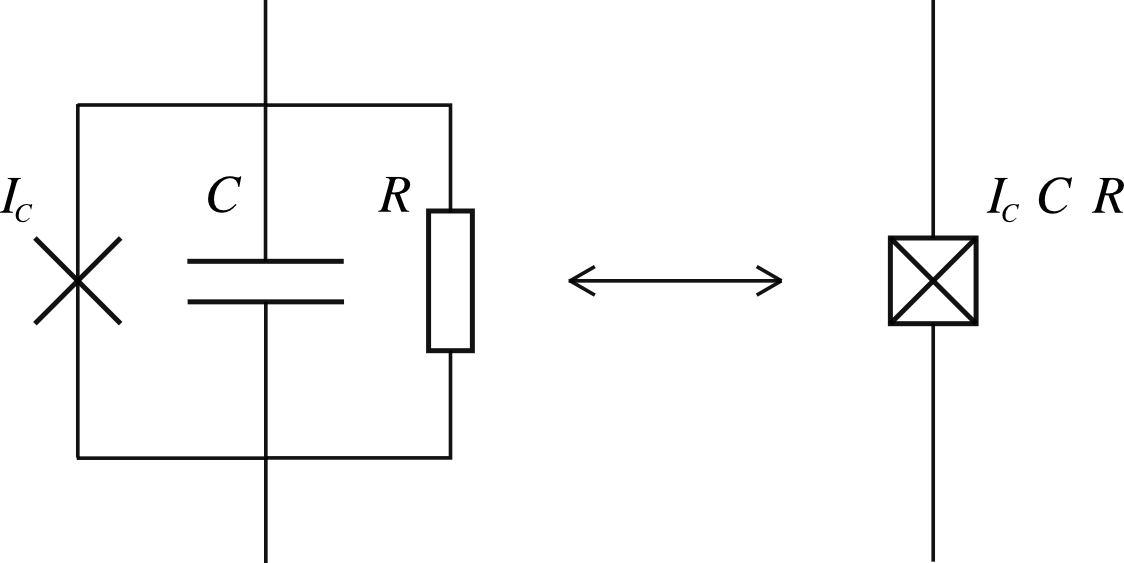
\includegraphics[width=1.05\textwidth]{RCSJ} 

RSCJ-модель
}
\only<2>{\vspace{1cm}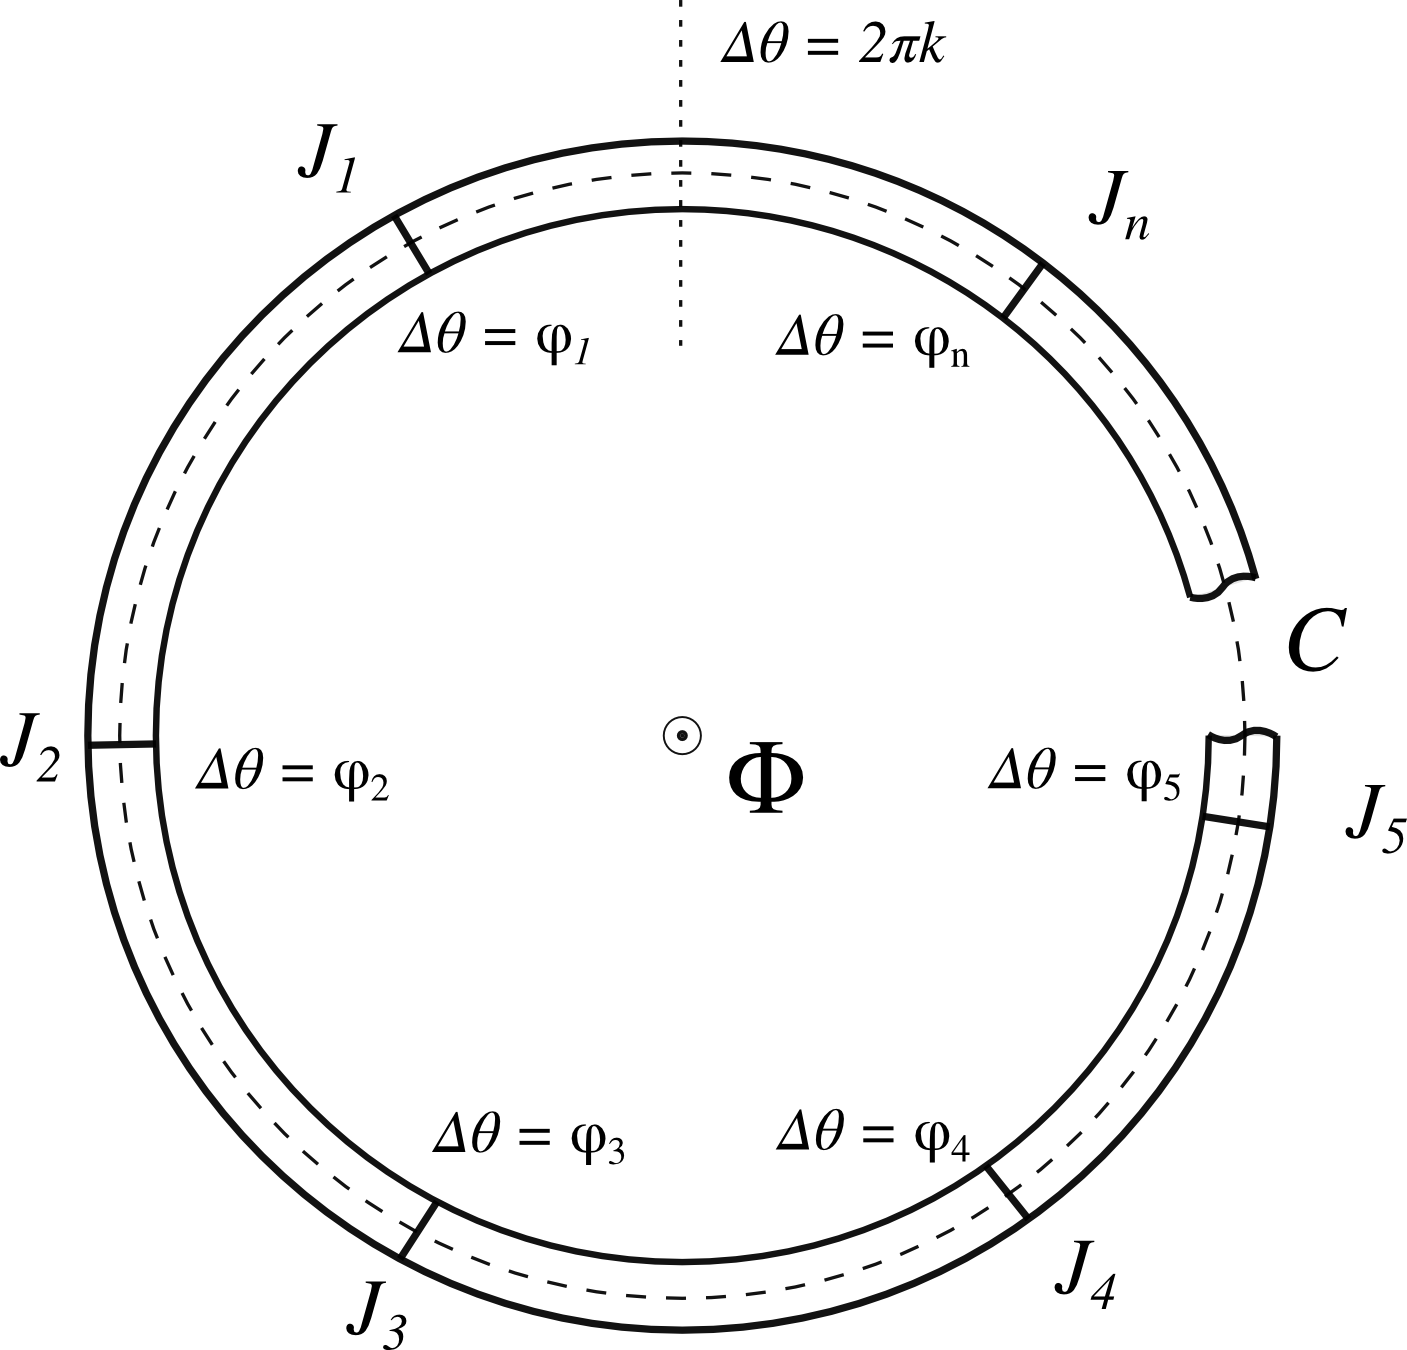
\includegraphics[width=0.9\textwidth]{ring}}
\end{columns}
\end{frame}

\subsection*{Гамильтониан Раби}
\begin{frame}[noframenumbering, c]\frametitle{\secname}\framesubtitle{\subsecname}

\centering
$\mathcal{\hat H}_R = \hat{\mathcal{H}}_{q}+\hat{\mathcal{H}}_{r}+\hat{\mathcal{H}}_{i}$
\vspace{1cm}
\begin{columns}[c]
	\begin{column}{.45\textwidth}
	\hspace{1cm}Из физической модели:
	\begin{align*}
	\hat{\mathcal{H}}_{q} &= \mathbbm{\hat 1}_r \otimes \left[\frac{\Delta}{2} \hat \sigma_x + 				\frac{\varepsilon}{2} \hat \sigma_z \right]\\
	\hat{\mathcal{H}}_{r} &= \hbar \omega_r \left(\frac{1}{2}+\hat a^\dag \hat a \right) \otimes \mathbbm{\hat 1}_q\\
	\hat{\mathcal{H}}_i &= g (\hat a^\dag + \hat a) \otimes \hat \sigma_z
	\end{align*}
	\end{column}

	\begin{column}{0.1\textwidth}
	{\huge $\overset{e^{i\frac{\pi}{4}\hat \sigma_y}}{\Rightarrow}$}
	\end{column}
	\begin{column}{.45\textwidth}
	\hspace{1.5cm}$\hat \sigma_x$ заменен на $\hat \sigma_z$:
	\begin{align*}
	\hat{\mathcal{H}}_{q} &= \mathbbm{\hat 1}_r \otimes \left[\frac{\Delta}{2} \hat \sigma_z + 				\frac{\varepsilon}{2} \hat \sigma_x \right]\\
	\hat{\mathcal{H}}_{r} &= \hbar \omega_r \left(\frac{1}{2}+\hat a^\dag \hat a \right) \otimes \mathbbm{\hat 1}_q\\
	\hat{\mathcal{H}}_i &= g (\hat a^\dag + \hat a) \otimes \hat \sigma_x
	\end{align*}
	\end{column}

\end{columns}
\end{frame}


\begin{frame}[noframenumbering, c]\frametitle{\secname}\framesubtitle{\subsecname}
\centering
$\mathcal{\hat H}_R = \hat{\mathcal{H}}_{q}+\hat{\mathcal{H}}_{r}+\hat{\mathcal{H}}_{i}$
\vspace{1cm}
\begin{columns}[c]
	\begin{column}{.4\textwidth}
	\hspace{1.5cm}$\hat \sigma_x$ заменен на $\hat \sigma_z$:
	\begin{align*}
	\hat{\mathcal{H}}_{q} &= \mathbbm{\hat 1}_r \otimes \left[\frac{\Delta}{2} \hat \sigma_z + 				\frac{\varepsilon}{2} \hat \sigma_x \right]\\
	\hat{\mathcal{H}}_{r} &= \hbar \omega_r \left(\frac{1}{2}+\hat a^\dag \hat a \right) \otimes \mathbbm{\hat 1}_q\\
	\hat{\mathcal{H}}_i &= g (\hat a^\dag + \hat a) \otimes \hat \sigma_x
	\end{align*}
	\end{column}

	\begin{column}{0.1\textwidth}	
	{\huge $\overset{e^{i\frac{\theta}{2}\hat \sigma_y}}{\Rightarrow}$}\\
	{\small $\tg \theta = \frac{\varepsilon}{\Delta}$}
	\end{column}
	
	\begin{column}{.5\textwidth}
	\hspace{1cm}конечная форма:
	\begin{align*}
	\hat{\mathcal{H}}_{q} &= \mathbbm{\hat 1}_r \otimes \frac{\hbar \omega_q}{2} \hat \sigma_z,\  \omega_q = \sqrt{\Delta^2+\varepsilon^2} \\
	\hat{\mathcal{H}}_{r} &= \hbar \omega_r  \left(\frac{1}{2}+\hat a^\dag \hat a \right) \otimes \mathbbm{\hat 1}_q\\
	\hat{\mathcal{H}}_i &= g (\hat a^\dag + \hat a) \otimes \left( \hat \sigma_x \sin\theta-  \hat\sigma_z \cos\theta \right)
	\end{align*}
	\end{column}
\end{columns}
\end{frame}

\subsection*{О приближениях}
\begin{frame}[noframenumbering, c]\frametitle{\secname}\framesubtitle{\subsecname}

\begin{block}{Без приближений:}
$\mathcal{\hat H}_i = g (\hat a^\dag + \hat a) \otimes \left( \hat \sigma_x \sin\theta-  \hat\sigma_z \cos\theta \right)$
\end{block}

\begin{block}{Стандартный RWA:}
$\mathcal{\hat H}_i = g \sin\theta \left(\hat a^\dag \otimes \hat \sigma^- + \hat a \otimes \hat \sigma^+\right) - g\cos\theta (\hat a^\dag + \hat a) \otimes \hat\sigma_z $
\end{block}

\begin{block}{Улучшенный RWA:}
$\mathcal{\hat H}_i = g \sin\theta \left(\hat a^\dag \otimes \hat \sigma^- + \hat a \otimes \hat \sigma^+\right) $
\end{block}

\end{frame}

\subsection*{Энергетический спектр модели Раби}
\begin{frame}[c, noframenumbering]\frametitle{\secname}\framesubtitle{\subsecname}
\begin{columns}
\only<1>{
\column{\textwidth}
\centering
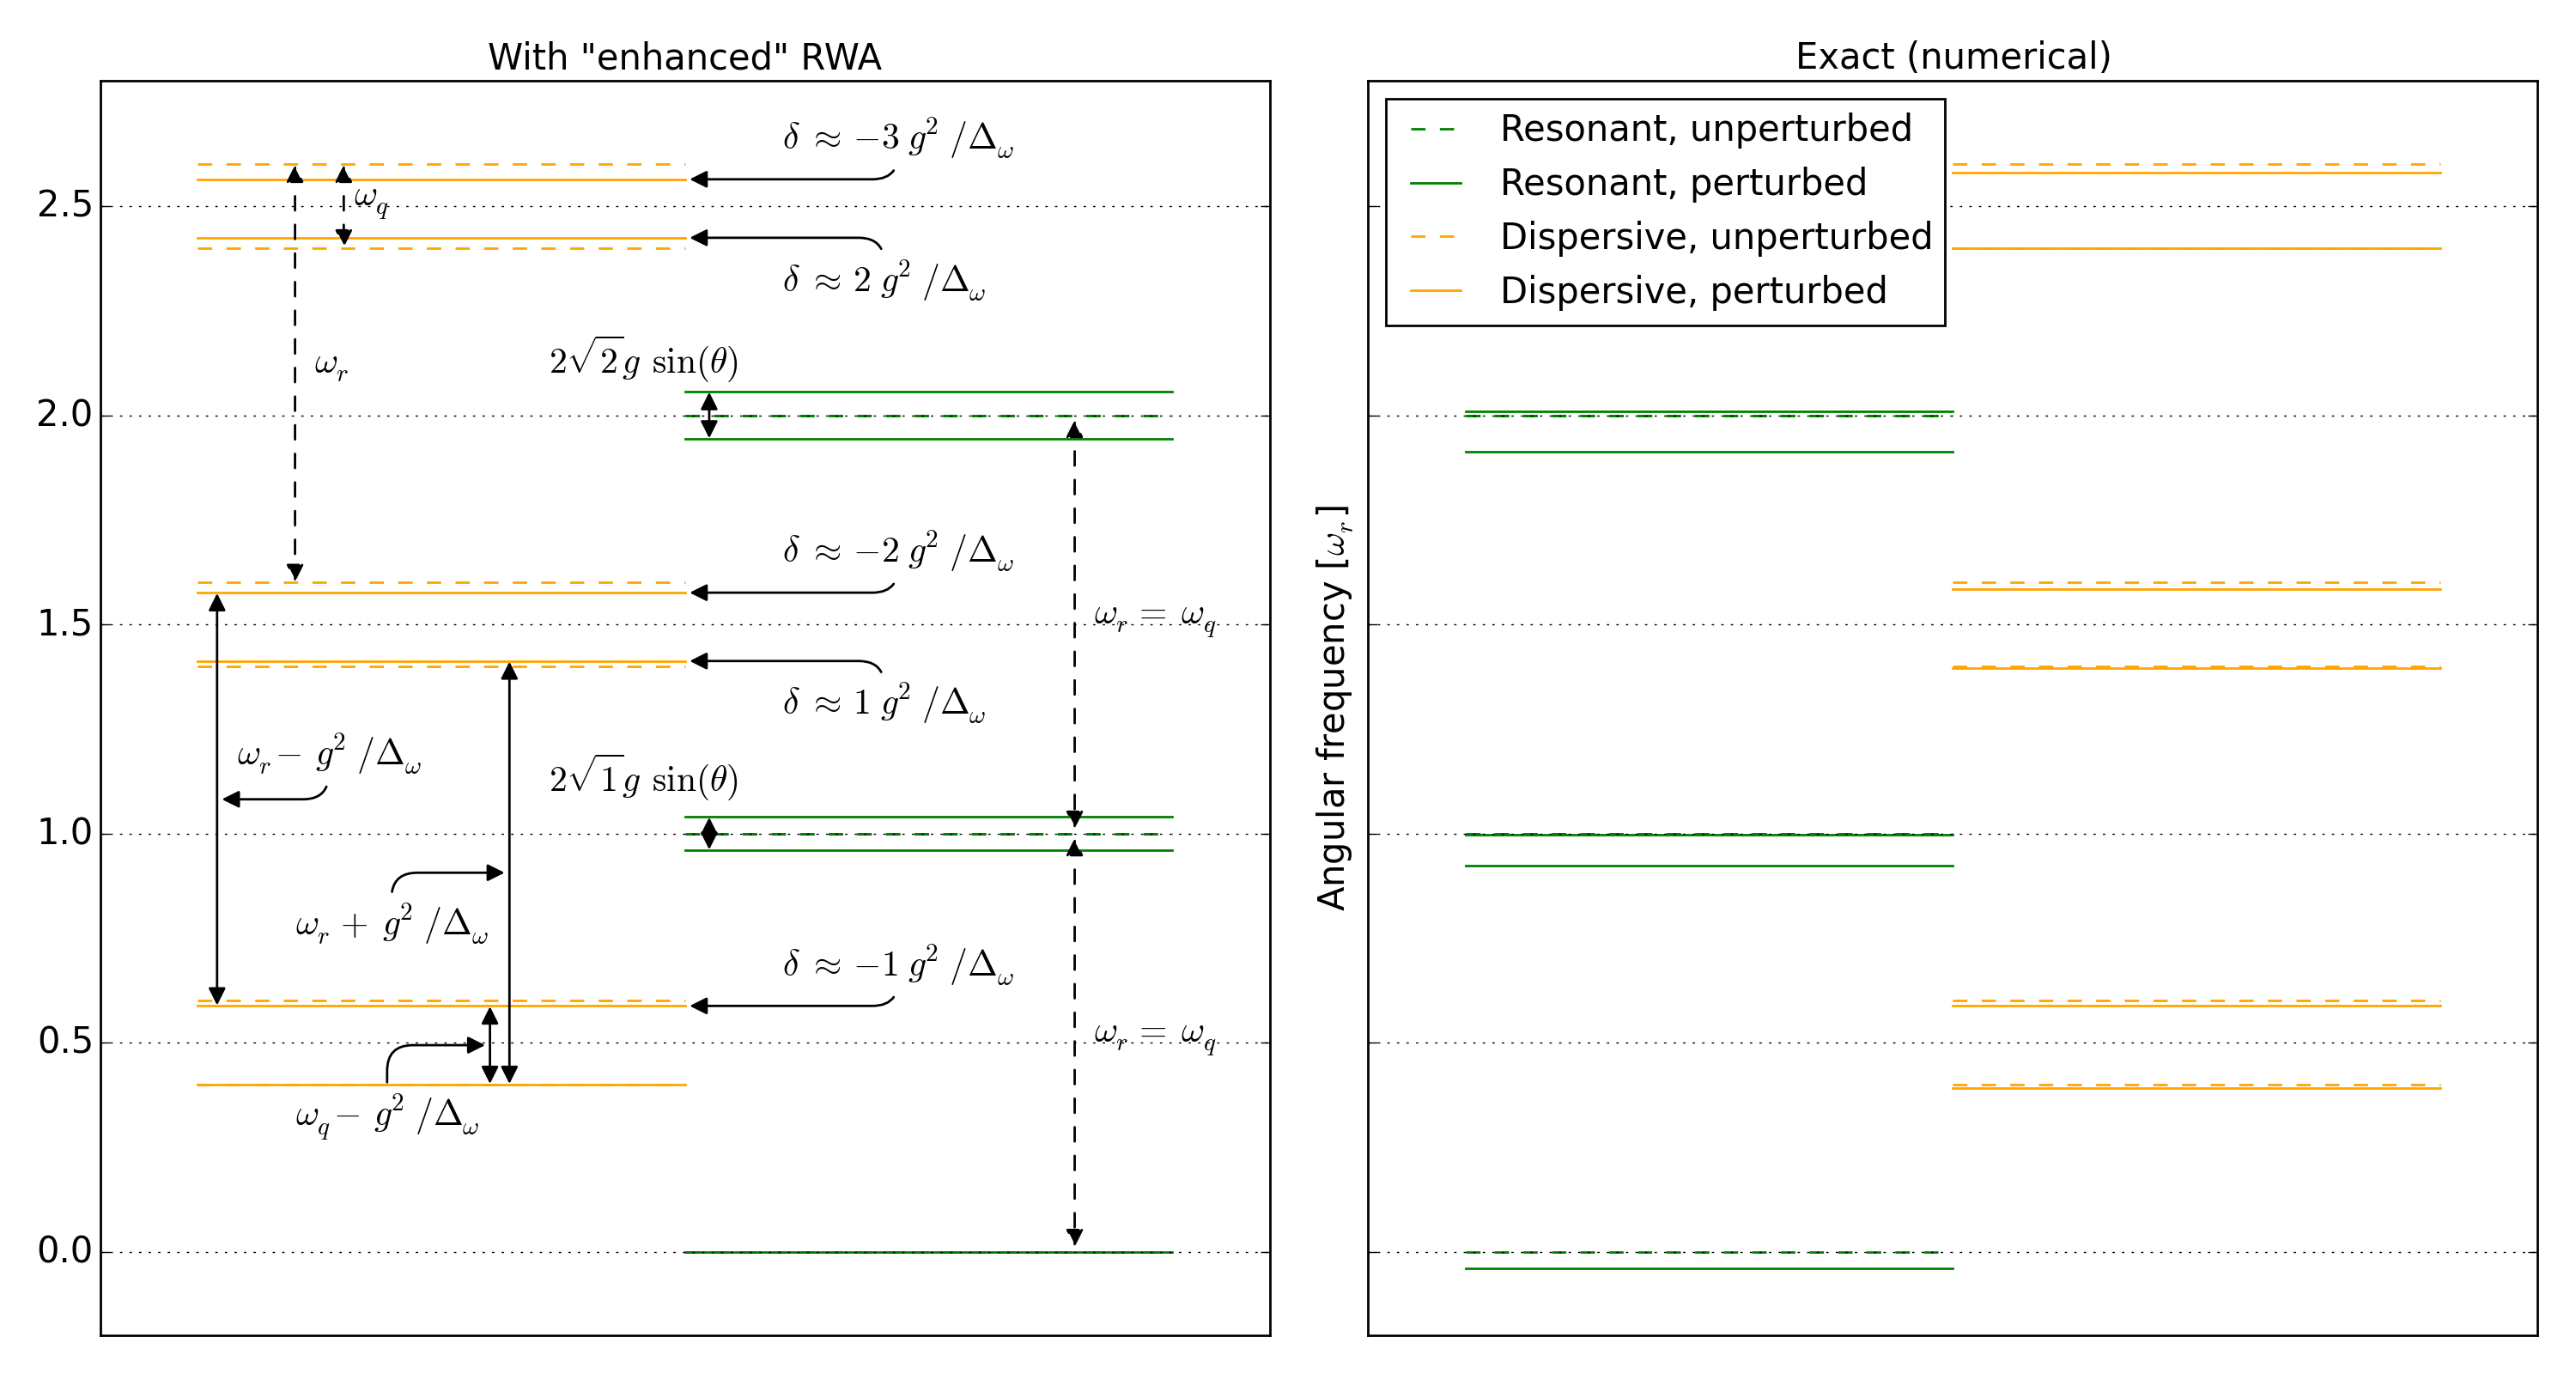
\includegraphics[width=1\textwidth]{JCM_levels}
}
\only<2>{
\column{0.5\textwidth}

\hspace{-1cm}
\centering
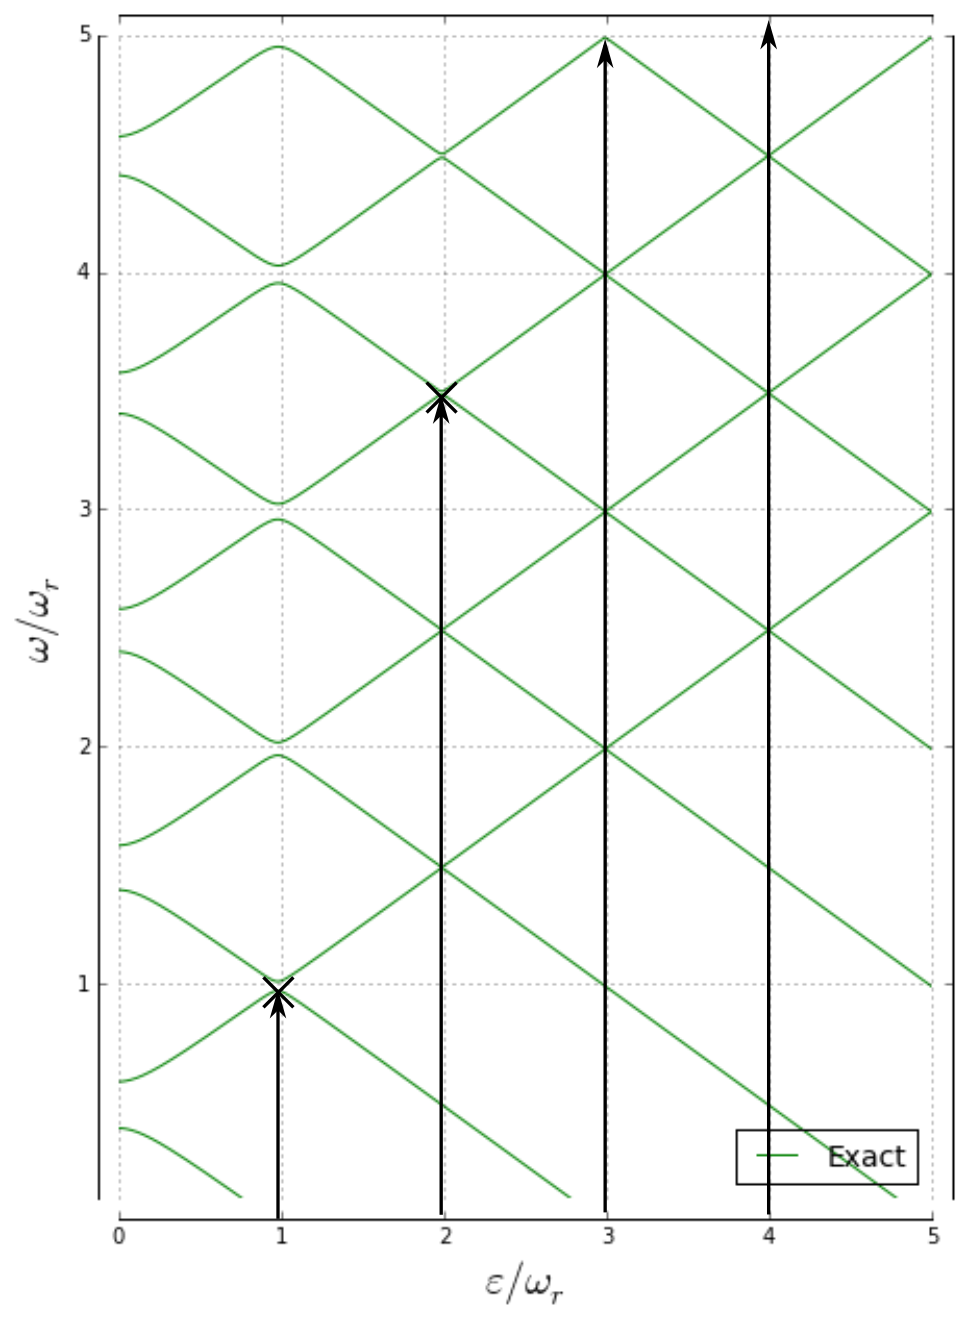
\includegraphics[height=0.8\textheight]{JCM_MF}
\column{0.5\textwidth}

\centering
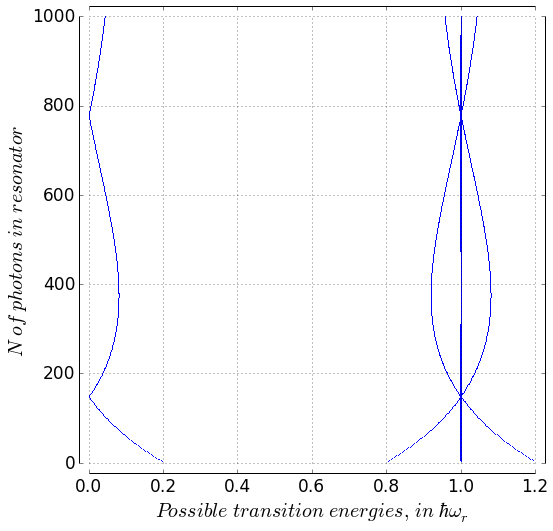
\includegraphics[height=0.8\textheight]{JCM_transitions}
}
\end{columns}
\end{frame}

\subsection*{Основное уравнение и теория отклика}
\begin{frame}[noframenumbering, c]\frametitle{\secname}\framesubtitle{\subsecname}
\begin{columns}[c]

\begin{column}{0.5\textwidth}
Основное уравнение форме Линдблада (T $\approx$ 0):
\begin{gather*}
i\hbar \frac{\partial}{\partial t}\hat \rho_s = \sbrkt{\mathcal{\hat H}_s, \hat \rho_s} + \\
+ \sum_{k=1}^3 \Gamma_k \rbrkt{\mathcal{\hat O}_k \hat \rho_s \mathcal{\hat O}_k^\dag - \frac{1}{2} \left\{ \mathcal{\hat O}_k^\dag \mathcal{\hat O}_k, \hat \rho_s \right\} } \\
\mathcal{\hat O}_1 = \hat a,\ \Gamma_1 = \kappa,\\
\mathcal{\hat O}_2 = \hat \sigma^-,\ \Gamma_2 = \gamma, \quad 
\mathcal{\hat O}_3 = \hat \sigma_z,\ \Gamma_3 = \gamma_\phi, \\
\mathcal{\hat H}_s = \mathcal{\hat H}_R + \text{driving}
\end{gather*}
\end{column}
\begin{column}{0.5\textwidth}
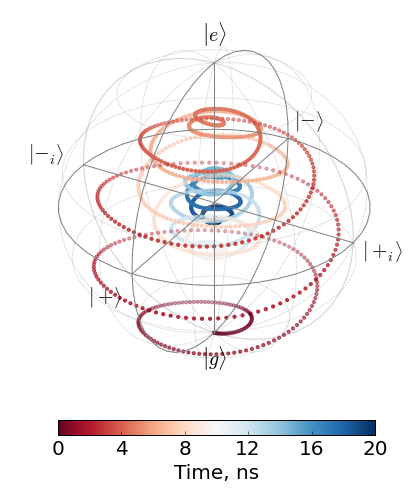
\includegraphics[width=0.9\textwidth]{rabi_dynamics_bloch_rel}
\end{column}
\end{columns}
\end{frame}

\begin{frame}[c]\frametitle{\secname}\framesubtitle{\subsecname}
Теория отклика:
\centering
\begin{equation*}
\mathcal{\hat H}_{tot} = \mathcal{\hat H}_{s} +\int d\omega\ \hbar \omega\, \hat b^\dag(\omega) \hat b(\omega) + \int d\omega\ [ \kappa(\omega) \hat c^{\dag} \hat b(\omega) + \kappa(\omega)\hat c \hat b^{\dag}(\omega)]
\end{equation*}

\begin{columns}[c]
\column{0.5\textwidth}
\begin{block}{Уравнение пропускания}
\centering
$\hat b_{out}= \sqrt{\gamma} \hat c,\quad \hat c \rightarrow \hat a \otimes \mathbbm{\hat 1}_q$\\

\vspace{.5cm}
$S_{21} \propto Tr\left[\hat \rho_s\ \hat a \otimes \mathbbm{\hat 1}_q\right]$
\end{block}
\column{0.5\textwidth}
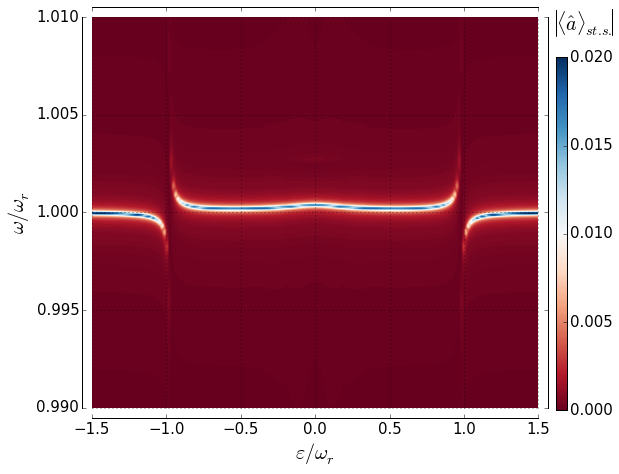
\includegraphics[width=0.9\textwidth]{Rabi_anticrossing_far_dyn}
\end{columns}
\end{frame}
\fi
\end{document}